\section{Data Modeling}
In this section, we first describe the collection of GSV images and the extraction of human-scale urban forms from the collected images.
Furthermore, we present the methods for data querying and filtering.

\begin{figure}[t]
	\centering
	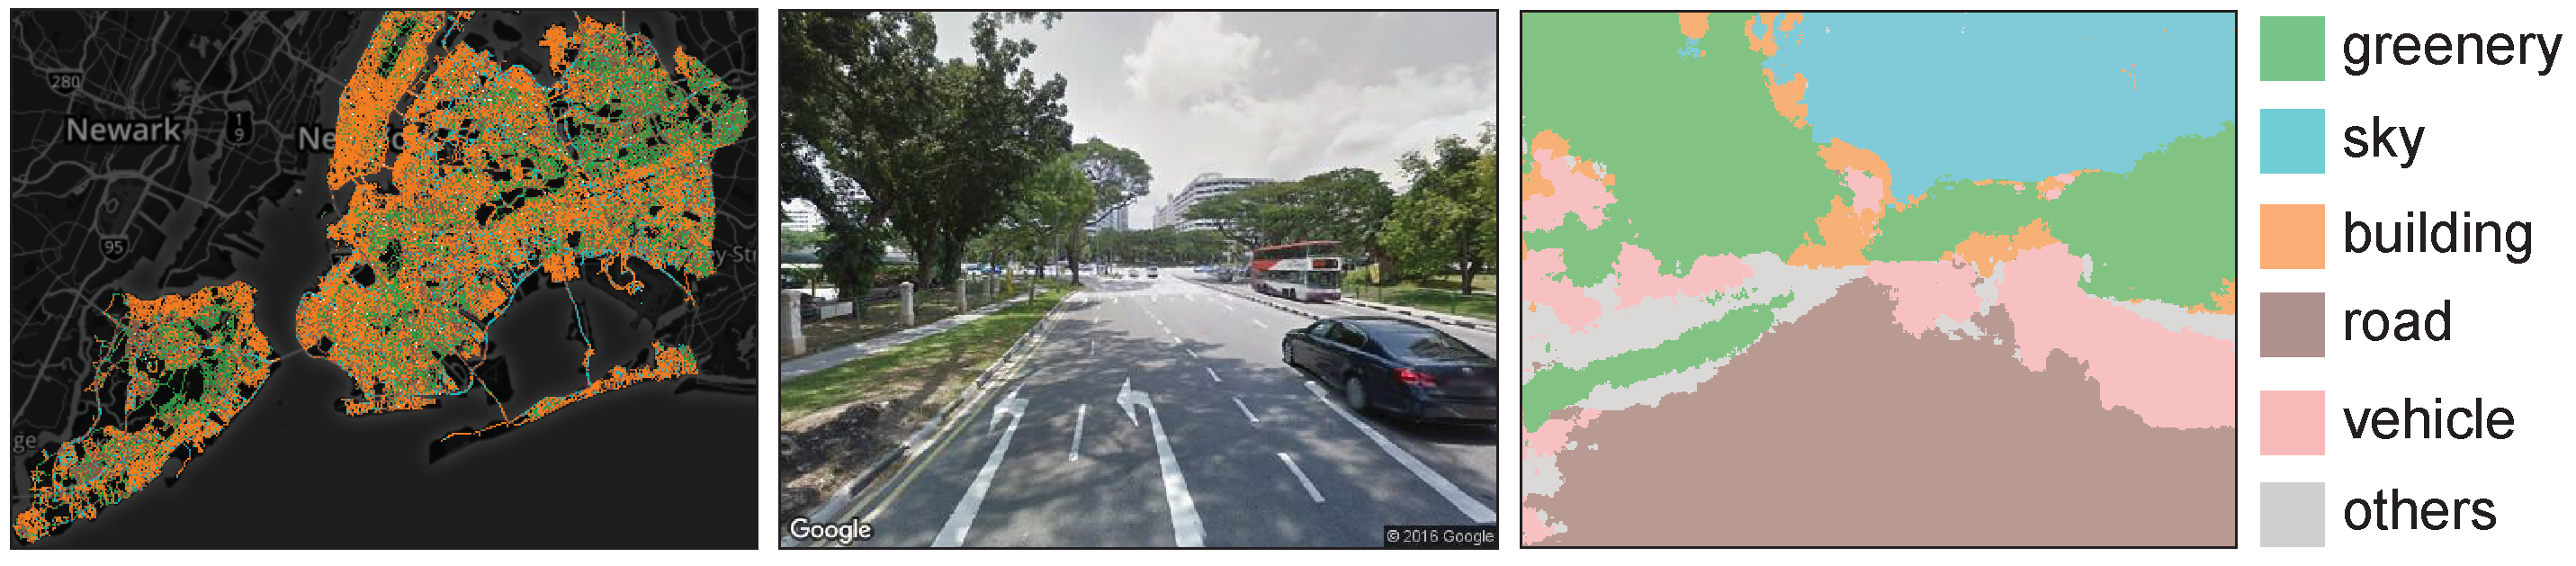
\includegraphics[width=\columnwidth]{figure/streetvizor/fig3_data_preprocess/data_process}
	\vspace{-7mm}
	\caption{Illustration of data preprocessing: sampling locations in New York City are generated from OpenStreetMap (left), a street view image is collected from Google Street View (center), and the image pixels are classified into six features using SegNet (right).}
	\label{fig:c1_data_preprocess}
	\vspace{-4mm}
\end{figure}

%===============================================
\subsection{Data Collection}
\label{ssec:c1_data_collection}

Based on the configurations defined in Section~\ref{sec:c1_bg}, we develop an automatic approach to collect GSV images.
We first download the area of a city from OSM~\cite{osm_api} and extract the road network from the OSM data.
Next, we apply a flood-fill algorithm that recursively goes through the entire road network every 50 meters, starting from a randomly selected location.
After this operation is completed, a list of sampling locations (\{$pos$\}) with geographic information $(lat \; \& \; long)$ is generated.
We then pass each $(lat \; \& \; long)$ into GSV API, and extract the corresponding street information $(SI)$, including street name $(s\_name)$ and heading $(h)$. 
Finally, we download front and back images at each sampling position by passing $lat, \; long \; \& \; h$ with the default field of view and pitch values into GSV API.
Together with the downloaded image ($Img$), we model urban forms at human-scale ($UF_{hs}$) at each sampling location as: 

\vspace*{-2mm}
\begin{equation}
\label{c1_eq_sv}
UF_{hs} \; := \; <pos, \; SI, \; Img>
\end{equation}

We have collected $\sim$147 k, $\sim$183 k, $\sim$685 k and $\sim$637 k images of Hong Kong, Singapore, Greater London and New York City, respectively.
Fig.~\ref{fig:c1_data_preprocess} (left) presents all sampling locations (colored dots) in New York City generated from OSM, and (center) shows a sample street view image downloaded from GSV.

%===============================================
\subsection{Feature Extraction}
\label{ssec:c1_feature}
After collecting street views, we first classify the image pixels into 12 classes (e.g., sky and building) using SegNet~\cite{Badrinarayanan_2015_segnet}, which is a robust pixel-wise semantic labeling tool with a global accuracy of 82.8\%.
Among the 12 classes, we count the number of pixels for the identified five features, i.e., $greenery$, $sky$, $building$, $road$, and $vehicle$, and summarize the remaining pixels as $others$.
We then normalize the feature data because pixel counts ($PC$) as raw output values are not intuitive.
The normalization is straightforward for each feature value ($FV$):
$ FV_i \; = {PC_i} / {PC_{Img}} $, where $i \in \{g, s, b, r, v, o\}$ represent the five features and $others$.
Hence, all feature values are in the range of [0, 1].
Then, we can replace the image ($Img$) with a feature metric ($FM$) as:

\vspace*{-2mm}
\begin{equation}
\label{c1_eq_fm}
Img \rightarrow FM := \; <FV_g, \; FV_s, \; FV_b, \; FV_r, \; FV_v, \; FV_o>
\end{equation}

% The feature extraction is preprocessed on a high-performance workstation with GTX 1080 graphics card. 
% Though enabled with GPU acceleration, the computation still takes from several to up to 20 hours to process the images in each city.
Fig.~\ref{fig:c1_data_preprocess} (right) shows the classification result of the street view image in the center produced by SegNet.

%===============================================
\subsection{Data Querying and Filtering}
\label{ssec:c1_query}

Based on Equations~\ref{c1_eq_sv} and~\ref{c1_eq_fm}, we model human-scale urban forms ($UF_{hs}$) with the following attributes: position ($pos$), street information ($SI$), and feature metric ($FM$).
By nature, the data exhibits the following properties: 
1) $spatial$, i.e., positions;
2) $multi$-$scale$, because the positions can be hierarchically grouped in accordance with city and regional units, or street information;
and 3) $multivariate$, i.e., the feature metric is in six-dimensional data space.

These complex data natures bring in challenges for our analytical tasks.
To address these challenges, we further identify the following querying and filtering models that our system should support:

\vspace*{-2mm}
\begin{itemize}

\item
\textbf{Spatial Query}:
To overview the feature distributions within an AOI (T.1.1), our system should first support an efficient query of a list of \{$UF_{hs}$\} with their $pos$ laying in a given AOI.
The AOI can be either an administrative zone (e.g., a city or a district) or a user-specified region defined using a lasso tool.
We achieve the efficient spatial query operation by organizing all \{$UF_{hs}$\} in a city in a four-level octree structure, in which the topmost level is the boundary of each city.

\vspace*{-2mm}
\item
\textbf{Street Query}:
To support the exploration of human-scale urban forms at street-scale (T.1.2), our system should allow users to interactively query a street by its name.
Here, we create a lookup table with street names as keys, and store corresponding $UF_{hs}$ ids in each street slot.

\vspace*{-2mm}
\item
\textbf{Feature Filtering}:
To accelerate filtering against a particular feature (T.2.2), our system first sorts all \{$UF_{hs}$\} to be explored in increasing order for every feature.
Then, we adopt a binary search approach in run time.

\end{itemize}

%===============================================
\begin{figure}[t]
	\centering
	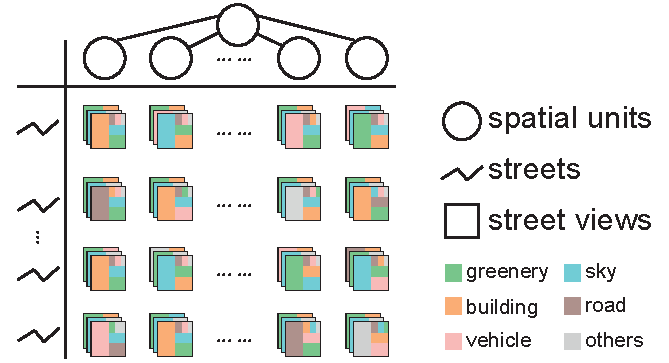
\includegraphics[width=0.8\columnwidth]{figure/streetvizor/fig4_data_model/data_model}
	\vspace{-3mm}
	\caption{Data model: street views with six-dimensional features of \textit{greenery, sky, building, road, vehicle} and \textit{others}, are organized in an octree structure and a street lookup table.}
	\vspace{-5mm}
	\label{fig:c1_data_model}
\end{figure}

\vspace*{-2mm}
Fig.~\ref{fig:c1_data_model} illustrates the data model that organizes the street views in an octree structure and a street lookup table.
Each street view contains the six-dimensional features of \textit{greenery, sky, building, road, vehicle}, and \textit{others}.
We store these querying and filtering models are stored in a back-end MongoDB database, as shown in Fig.~\ref{fig:c1_sys_overview}.
%===============================================
